\chapter{The incident beam}
\label{ch:beam}

\section{What it does}

The module \code{beam.py} chooses the point $(x,y)$ of the beam rectangle where each particle starts. Its main
function is
\begin{lstlisting}
sample_beam_point(width, height, H=None, V=None, n=1, rng=None)
\end{lstlisting}
\begin{description}
  \item[\code{width}, \code{height}] size of the beam along $x$ and $y$, in mm.
  \item[\code{H}, \code{V}] optional functions $H(x)$ and $V(y)$ (with $x$ and $y$ in mm) giving the relative intensity
        across the beam. They need not be normalised; they must be non-negative. By default both are uniform.
  \item[\code{n}] number of particles. With \code{n=1} the result is a pair of numbers; otherwise a pair of arrays.
  \item[\code{rng}] seed or random generator.
\end{description}
The result is the start point in mm, relative to the centre of the beam: $x\in[-w_b/2,\,w_b/2]$ and
$y\in[-h_b/2,\,h_b/2]$. The two profiles are treated as independent, so the intensity map is $H(x)\,V(y)$.
The function \code{start_position} returns the same point as a three-dimensional position together with the direction
of flight $(0,0,1)$.

\section{Method: inverse transform sampling}

For a uniform profile, the position is a uniform random number in the interval. For any other profile the
function uses \emph{inverse transform sampling}. The profile $f(x)$ is evaluated on a fine grid, and its cumulative
distribution
\begin{equation}
  F(x) = \frac{\int_{-w_b/2}^{x} f(x')\,\deriv{x'}}{\int_{-w_b/2}^{w_b/2} f(x')\,\deriv{x'}}
\end{equation}
is computed with the trapezoidal rule. If $u$ is a random number uniform between 0 and 1, then $x=F^{-1}(u)$ is distributed
according to $f$: where the profile is high $F$ grows fast, so many values of $u$ are mapped to that region. The inverse is
read with \code{np.interp}. This method needs neither the maximum of the profile nor rejected points.

\section{Example}

\pyexample{ex01_beam}

Figure~\ref{fig:beam} shows 6000 start points of a $10\times6$~mm beam with a Gaussian horizontal profile
($\sigma=1.5$~mm) and a uniform vertical profile.

\begin{figure}[ht]
  \centering
  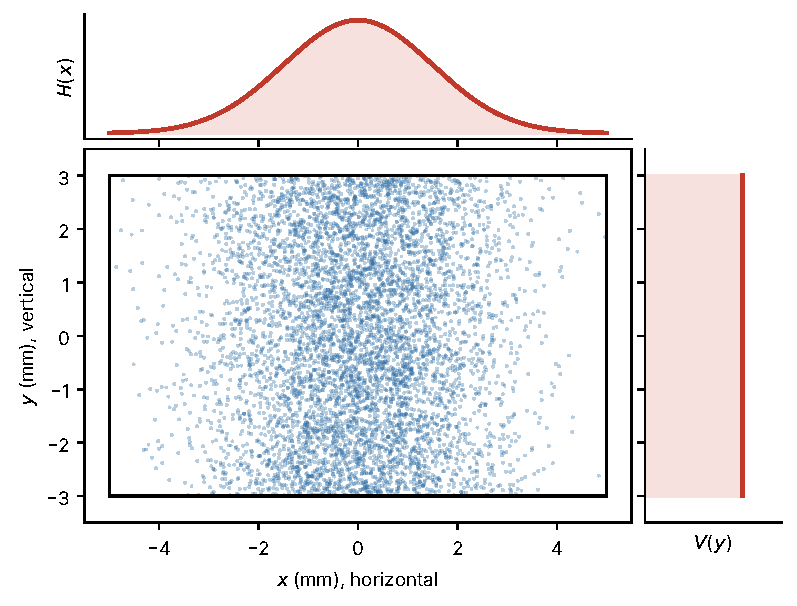
\includegraphics[width=0.75\textwidth]{fig_beam}
  \caption{Start points of the particles in a beam $10\times6$~mm with a Gaussian $H(x)$ ($\sigma=1.5$~mm) and a uniform $V(y)$.
  The curves are the profiles.}
  \label{fig:beam}
\end{figure}

A profile can be any function that accepts a NumPy array, for instance a measured profile interpolated with
\code{np.interp}:
\begin{lstlisting}
x_measured = np.array([-4, -2, 0, 2, 4]);  I_measured = np.array([0, 0.5, 1, 0.5, 0])
H = lambda x: np.interp(x, x_measured, I_measured)
xs, ys = sample_beam_point(8, 6, H=H, n=10000)
\end{lstlisting}
If a profile only accepts single numbers, the function calls it once per grid point.
